\documentclass{article} % For LaTeX2e
\usepackage{nips15submit_e,times}
\usepackage{hyperref}
\usepackage{url}
\usepackage{bm, subfigure}
\usepackage{inputenc}
\usepackage{amsmath,amssymb,amsthm}
\usepackage{amsthm}
\usepackage{algorithm, algorithmic}
\usepackage{graphicx}
\usepackage[backgroundcolor=white,linecolor=red,bordercolor=white,textsize=tiny,textwidth=10mm]{todonotes}

\newcommand{\ica}{\hspace{0.25cm}}
\renewcommand{\arraystretch}{0.94}

\DeclareMathOperator*{\argmin}{arg\,min}
\DeclareMathOperator*{\argmax}{arg\,max}


%\documentstyle[nips14submit_09,times,art10]{article} % For LaTeX 2.09


\newtheorem{theorem}{Theorem}
\mathchardef\mhyphen="2D

\title{Stochastic Expectation Propagation}


\author{
Yingzhen Li \\
Department of Engineering\\
University of Cambridge\\
Cambridge, CB2 1PZ, UK \\
\texttt{yl494@cam.ac.uk} \\
\And
Miguel to enter details\\
\And
Richard E.~Turner \\
Affiliation \\
Address \\
\texttt{ret26@cam.ac.uk} \\
}

% The \author macro works with any number of authors. There are two commands
% used to separate the names and addresses of multiple authors: \And and \AND.
%
% Using \And between authors leaves it to \LaTeX{} to determine where to break
% the lines. Using \AND forces a linebreak at that point. So, if \LaTeX{}
% puts 3 of 4 authors names on the first line, and the last on the second
% line, try using \AND instead of \And before the third author name.

\newcommand{\fix}{\marginpar{FIX}}
\newcommand{\new}{\marginpar{NEW}}

%\nipsfinalcopy % Uncomment for camera-ready version

\begin{document}


\maketitle

%%%%%%%%%%%%%%%%%%%%%%%%%%%%%%%%%%%%%%%%%
\begin{abstract}
Expectation propagation (EP) is a deterministic approximation algorithm that is often used to perform approximate Bayesian parameter learning. EP approximates the full intractable posterior distribution through a set of local-approximations that are iteratively refined for each datapoint. EP can offer analytic and computational advantages over other approximations, such as Variational Inference (VI), and is the method of choice for a number of models \cite{can we have citations}. The local nature of EP appears to make it an ideal candidate for performing Bayesian learning on large-scale datasets. However, EP has a crucial limitation in this context: the number approximating factors need to increase with the number of data-points, $N$, which entails a large computational burden. This paper presents an extension to EP, called stochastic expectation propagation (SEP), that maintains a global posterior approximation (like VI) but updates it in a local way (like EP).  Experiments on a number of synthetic and real-world data indicate that SEP performs almost as well as full EP, but reduces the memory consumption by a factor of $N$. 
\end{abstract}


%%%%%%%%%%%%%%%%%%%%%%%%%%%%%%%%%%%%%%%%%%
%%%% INTRODUCTION
\section{Introduction}


Recently a number of methods have been developed for applying Bayesian learning to large datasets. Examples include sampling such as \cite{ahn:distributedMCMC, bardenet:MCMC}, distributional approximations including stochastic variational inference (SVI) \cite{hoffman:svi} and assumed density filtering (ADF) \cite{miguel:pbp}, and approaches that mix distributional and sampling approximations \cite{gelman:dep,xu:sms}. 
%
One family of approximation method has garnered less attention in this regard: expectation propagation (EP) \cite{minka:ep, opper:ec}. EP constructs a posterior approximation by iterating simple local computations that refine factors which approximate the posterior-contribution from each datapoint. At first sight, it therefore appears well suited to large-data problems: the locality of computation make the algorithm simple to parallelise and distribute, and good practical performance on a range of small-data applications suggest that it will be accurate \cite{kuss:gpep,barthelme:ep_likelihood,cunningham:gaussianEP}. 
%
\hl{However the elegance of local computation has been bought at the price of prohibitive memory overhead that grows with the number of datapoints $N$, since each local approximating factor typically has the same complexity as the global approximation. The same pathology exists for the broader class of power EP (PEP) algorithms } \cite{minka:powerep} \hl{that includes variational message passing} \cite{winn:vmp}. \hl{In contrast, variational inference (VI) methods} \cite{jordan:variational,beal:variational} \hl{utilise global approximations that are refined directly, which prevents memory overheads from scaling with $N$. }

%On the other hand, there is a critical computational bottleneck in the standard EP approximation: each local approximating factor typically has the same complexity as the global approximation. This means that the EP algorithm has a memory overhead that grows with the number of data-points $N$, which makes it hard to scale rich models with many parameters to large-data settings (consider approximating the posterior distribution of a topic model with millions of parameters on a corpus containing billions of documents). The same pathology exists for the broader class of power EP (PEP) algorithms \cite{minka:powerep} that includes variational message passing \cite{winn:vmp}. The elegance of local computation has been bought at the price of having myriad local approximating factors. In contrast, variational inference (VI) methods \cite{jordan:variational,beal:variational} utilise global approximations that are refined directly (rather than through local components) which prevents memory overheads from scaling with $N$. 

Is there ever a case for preferring EP (or PEP) to VI methods for large-data?  We believe that there certainly is. First, EP can provide significantly more accurate approximations. It is well known that variational free-energy approaches are biased and often severely so \cite{turner+sahani:2011a} and for particular models the variational free-energy objective is pathologically ill-suited \cite{cunningham:gaussianEP,turner+sahani:2011c}. Second, the fact that EP is truly local (to factors in the posterior distribution and not just likelihoods) means that it affords different opportunities for tractable algorithm design, as the updates can be simpler to approximate.
%(the probabilistic back-propagation setting treated later in the paper is one such case where PEP is tractable, but variational free-energy methods require a second level of approximation\todo[fancyline]{double check with Miguel that this is correct}). 

As EP appears to be the method of choice for some applications, researchers have attempted to push it to scale. One approach is to swallow the large computational burden and simply use large data-structures to store the approximating factors (e.g.~TrueSkill \cite{herbrich:trueskill}). This approach can only be pushed so far. A second approach is to use \hl{ADF as a simple variant}, %of EP called assumed density filtering (ADF) 
which only requires a global approximation to be stored \cite{maybeck:adf}. ADF, however, provides poorly calibrated uncertainty estimates \cite{minka:ep} which was one of the main motivating reasons for developing EP in the first place. 
A third idea, complementary to the one described here, is to use approximating factors that have simpler structure (e.g.~low rank, \cite{qi+minka:sparseGP}). This reduces memory consumption (e.g.~for Gaussian factors from $\mathcal{O}(ND^2)$ to $\mathcal{O}(ND)$), but does not stop the scaling with $N$. Another idea uses EP to carve up the dataset \cite{gelman:dep,xu:sms} using approximating factors for collections of data-points. This results in coarse-grained, rather than local, updates and other methods must be used to compute them. (Indeed, the spirit of \cite{gelman:dep,xu:sms} is to extend sampling methods to large-datasets, not EP itself.) 

\hl{Can we have the best of both worlds? That is, accurate global approximations that are derived from truly local computation. To address this question we develop an algorithm based upon the standard EP and ADF algorithms that maintains a global approximation which is updated in a local way.}
%The question addressed in this paper is: can we have the best of both worlds? That is, accurate global approximations that are derived from truly local computation. For this purpose we develop an algorithm based upon the standard EP and ADF algorithms that maintains a global approximation which is updated in a local way. 
%
We call this class of algorithms stochastic expectation propagation (SEP) since it updates the global approximation with (damped) stochastic estimates on data sub-samples in an analogous way to SVI. Indeed, the generalisation of the algorithm to the PEP setting directly relates to SVI. 
%
\hl{Importantly, SEP reduces the memory footprint by a factor of $N$ when compared to EP. We further extend the method to control the granularity of the approximation, and to treat models with latent variables without compromising on accuracy or unnecessary memory demands. Finally, we demonstrate the scalability and accuracy of the method on a number of real world and synthetic datasets.}

%Tests on synthetic data indicate that SEP performs almost as well as full EP, but reduces the memory footprint by a factor of $N$, and that it has well calibrated uncertainty estimates, unlike ADF. We show how to extend the method to treat models with latent variables without compromising on accuracy or memory demands. Finally, we demonstrate the scalability and accuracy of the method on a number of real world and synthetic datasets.




%%%%%%%%%%%%%%%%%%%%%%%%%%%%%%%%%%%%%%%%%%%%
%%%%% SECTION 2: EP, ADF & SEP %%%%%%%%%%%%


\section{Expectation Propagation and Assumed Density Filtering}
%short review on EP
We begin by briefly reviewing the EP and ADF algorithms upon which our new method is based. Consider for simplicity observing a dataset comprising $N$ i.i.d.~samples $\mathcal{D} = \{\bm{x}_n \}_{n=1}^N$ from a probabilistic model $p(\bm{x}|\bm{\theta})$ parametrised by an unknown $D$-dimensional vector $\bm{\theta}$ that is drawn from a prior $p_0(\bm{\theta})$. Exact Bayesian inference involves computing the (typically intractable) posterior distribution of the parameters given the data, 
\begin{equation}
p(\bm{\theta} | \mathcal{D}) \propto p_0(\bm{\theta}) \prod_{n=1}^{N} p(\bm{x}_n | \bm{\theta}) \approx q(\bm{\theta}) \propto p_0(\bm{\theta}) \prod_{n=1}^{N} f_n(\bm{\theta}).
\end{equation}
%
Here $q(\bm{\theta})$  is a simpler tractable approximating distribution that will be refined by EP.
%
% and from a distribution family $\mathcal{P}$, is introduced to estimate the underlying data distribution. Bayesian methods require posterior computation after observing dataset $D = \{\bm{x}_i \}_{i=1}^N$ using Bayes Rule: 
%\begin{equation}
%p(\bm{\theta} | D) \propto p_0(\bm{\theta}) \prod_{i=1}^{N} p(\bm{x}_i | \bm{\theta}),
%\end{equation}
%however this posterior is often in some intractable family $\tilde{\mathcal{P}}$ for many powerful probabilistic models. Expectation propagation approximates the true posterior with a suitable distribution $q(\bm{\theta}) \in \mathcal{Q}$, which factorises over likelihood terms
%
%\begin{equation}
%q(\bm{\theta}) \propto p_0(\bm{\theta}) \prod_{n=1}^{N} f_n(\bm{\theta}).
%\end{equation}
%
The goal of EP is to refine the approximate factors so that they capture the contribution of each of the likelihood terms to the posterior i.e.~$f_n(\bm{\theta}) \approx p(\bm{x}_n | \bm{\theta})$. In this spirit, one approach would be to find each approximating factor $f_n(\bm{\theta})$ by minimising the Kullback Leibler (KL) Divergence between the posterior and the distribution formed by replacing one of the likelihoods by its corresponding approximating factor,  $\mathrm{KL}[p(\bm{\theta}|\mathcal{D}) || p(\bm{\theta}|\mathcal{D}) f_n(\bm{\theta})/ p(\bm{x}_n | \bm{\theta})]$. Unfortunately, such an update is still intractable as it involves computing the full posterior. Instead, EP approximates this procedure by replacing the exact leave-one-out posterior $p_{-n}(\bm{\theta}) = p(\bm{\theta}|\mathcal{D}) / p(\bm{x}_n | \bm{\theta})$ on both sides of the KL by the approximate leave-one-out posterior (called the cavity distribution) $q_{-n}(\bm{\theta}) =q(\bm{\theta})/f_n(\bm{\theta})$. Since this couples the updates for the approximating factors, the updates must now be iterated.

In more detail, EP iterates four simple steps. First, the factor selected for update is removed from the approximation to produce the cavity distribution. Second, the corresponding likelihood is included to produce the tilted distribution $\tilde{p}_n(\bm{\theta}) = q_{-n}(\bm{\theta}) p(\bm{x}_n | \bm{\theta})$. Third EP updates the approximating factor by minimising $\mathrm{KL}[\tilde{p}_n(\bm{\theta}) || q_{-n}(\bm{\theta})  f_n(\bm{\theta})]$. The hope is that the contribution the true-likelihood makes to the posterior is similar to the effect the same likelihood has on the tilted distribution. If the approximating distribution is in the exponential family, as is often the case, then the KL minimisation reduces to a moment-matching step \cite{amari:ig} that we denote $f_n(\bm{\theta}) \leftarrow \mathtt{proj}[\tilde{p}_n(\bm{\theta})] / q_{-n}(\bm{\theta}) $. Finally, having updated the factor, it is included into the approximating distribution.\todo[fancyline]{mention damping here?}
%
%Next EP updates the  $\mathrm{KL}(p(\bm{\theta})||q(\bm{\theta}))$
%
% is removed from the approximating distribution
%
%
%by matching the moments of the corresponded single datapoint posterior. To be precise, an EP iteration begins with removing the selected factor $f_i(\bm{\theta})$ to form the cavity distribution $q_{-i}(\bm{\theta})$, then uses it as the prior distribution to incorporate the current likelihood $p(\bm{x}_i| \bm{\theta})$. The local posterior $\tilde{p}_i(\bm{\theta}) \propto p(\bm{x}_i|\bm{\theta}) q_{-i}(\bm{\theta})$ is also referred as the tilted distribution, which is in the $\tilde{\mathcal{P}}$ family as well. 
%
%Next EP proposes a moment projection (M-projection) \cite{amari:ig} or moment matching step to approximate the tilted distribution by minimising $KL(p(\bm{\theta})||q(\bm{\theta}))$ wrt.~$q(\bm{\theta})$, and finally recovers the new updates of the current factor $f_i(\bm{\theta}) \buildrel\propto\over \leftarrow q(\bm{\theta}) / q_{-1}(\bm{\theta})$.

We summarise the update procedure for a single factor in Algorithm \ref{alg:ep}. Critically, the approximation step of EP involves local computations since one likelihood term is treated at a time. The assumption is that these local computations, although possibly requiring further approximation, are far simpler to handle compared to the full posterior $p(\bm{\theta}| \mathcal{D})$. In practice, EP often performs well when the updates are parallelised. Moreover, by using approximating factors for groups of data-points, and then running additional approximate inference algorithms to perform the EP updates (which could include nesting EP), EP carves up the dataset meaning it is a good candidate for distributed approximate inference.\todo[fancyline]{Mention full factor graph interpretation, message passing? theory available for EP here? fixed point properties, marginal likelihood?}

% ADF
There is, however, one wrinkle that complicates deployment of EP at scale. Computation of the cavity distribution requires removal of the current approximating factor and this means that any implementation of EP must store them explicitly necessitating an $\mathcal{O}(N)$ memory footprint. One option is to simply ignore the removal step replacing the cavity distribution with the full approximation resulting in the ADF algorithm (see Algorithm \ref{alg:adf}). ADF has the advantage that only the global approximation need be maintained in memory, but as the moment matching step now over-counts the underlying approximating factor (consider the new form of the objective $\mathrm{KL}[q(\mathbf{\theta}) p(\bm{x}_n | \bm{\theta}) || q(\bm{\theta})]$) the variance of the approximation shrinks to zero as multiple passes are made through the dataset. Early stopping is therefore required to prevent overfitting and generally speaking ADF does not uncertainties that are well-calibrated to the posterior. 

In the next section we introduce a new algorithm that sidesteps EP's large memory demands whilst avoiding the pathological behaviour of ADF. 

\section{Stochastic Expectation Propagation}
%
% SEP
In this section we introduce a new algorithm, inspired by EP, called SEP that combines the benefits of local approximation (including tractability of updates, distributability, and parallelisability) with global approximation (reduced memory demands).  The algorithm can be interpreted as a version of EP in which the approximating factors are tied, or alternatively as a corrected version of ADF that prevents overfitting. 

The key idea is that, at convergence, the approximating factors in EP can be interpreted as parameterising a global factor,  $f(\bm{\theta})$, that captures the average effect of a likelihood on the posterior  $\prod_{n=1}^{N} f_n(\bm{\theta}) = f(\bm{\theta})^{N} \approx \prod_{n=1}^{N} p(\bm{x}_n | \bm{\theta})$. In this spirit, the new algorithm employs direct iterative refinement of a global approximation comprising the prior and $N$ copies of a single approximating factor, $f(\bm{\theta})$, $q(\bm{\theta}) \propto f(\bm{\theta})^N p_0(\bm{\theta})$.
%EP has been shown very successful in previous investigations as mentioned, however very little work has been done on large datasets due to its large memory consumption. It requires the program to store every local approximator $f_i(\bm{\theta})$, resulting in space complexity $\mathcal{O}(Nd^2)$ if using Gaussians. To eliminate the linear factor $N$ in the storage requirement, we propose a factor-tying approach by defining a new approximation structure
%
%\begin{equation}
%q(\bm{\theta}) \propto f(\bm{\theta})^N p_0(\bm{\theta}).
%\end{equation}
%
%The goal is to refine $f(\bm{\theta})$ in such a way that it captures the average effect a likelihood function has on the posterior. 
SEP uses updates that are analogous to EP's in order to refine $f(\bm{\theta})$ in such a way that it captures the average effect a likelihood function has on the posterior. First the cavity distribution is formed by removing one of the copies of the factor, $q_{-n}(\bm{\theta}) =q(\bm{\theta})/f(\bm{\theta})$. 
Second, the corresponding likelihood is included to produce the tilted distribution $\tilde{p}_n(\bm{\theta}) = q_{-1}(\bm{\theta}) p(\bm{x}_n | \bm{\theta})$ and, third, EP finds an intermediate factor approximation by moment matching, $f_n(\bm{\theta}) \leftarrow \mathtt{proj}[\tilde{p}_n(\bm{\theta})] / q_{-1}(\bm{\theta}) $. Finally, having updated the factor, it is included into the approximating distribution. It is important here not to make a full update since $f_n(\bm{\theta})$ captures the effect of just a single likelihood function  $p(\bm{x}_n | \bm{\theta})$. Instead, damping should be employed to make a partial update $f(\bm{\theta}) \leftarrow f(\bm{\theta})^{1 - \alpha} f_n(\bm{\theta})^{\alpha}$ a natural choice uses $\alpha = 1/N$ which can be interpreted as minimising  $\mathrm{KL}[\tilde{p}_n(\bm{\theta}) || p_{0}(\theta)  f(\bm{\theta})^N]$ in the moment update.

SEP is summaried in Algorithm \ref{alg:sep}. Unlike ADF, the cavity is formed by dividing out $f(\bm{\theta})$ which captures the average affect of the likelihood and prevents the posterior from collapsing. Like ADF, however, memory allocation for $f(\bm{\theta})$ is unnecessary because it can be recovered from the approximate posterior, $f(\bm{\theta}) \propto (q(\bm{\theta}) / p_0(\bm{\theta}))^{\frac{1}{N}}$ and $q_{-1}(\bm{\theta}) \propto q(\bm{\theta})^{1 - \frac{1}{N}} p_0(\bm{\theta})^{\frac{1}{N}}$. When Gaussian approximating factors are used, for example, SEP reduces the storage requirement of EP from  $\mathcal{O}(NK^2)$ to $\mathcal{O}(K^2)$ which is a substantial saving that enables models with many parameters to be applied to large datasets. 

\begin{figure}[!t]
% UGLY USE OF \vspace & \hspace follows
\begin{minipage}[t]{0.33\linewidth}
\centering
\begin{algorithm}[H] 
\caption{EP} \small
\label{alg:ep} 
\begin{algorithmic}[1] 
	\STATE choose a factor $f_n$ to refine:
	\STATE compute cavity distribution \\$q_{-n}(\bm{\theta}) \propto q(\bm{\theta}) / f_n(\bm{\theta})$ 
	\STATE compute tilted distribution \\$\tilde{p}_n(\bm{\theta}) \propto p(\bm{x}_n|\bm{\theta}) q_{-n}(\bm{\theta})$
	\STATE moment matching: \\ \hspace{-1mm}$f_n(\bm{\theta}) \leftarrow \mathtt{proj}[\tilde{p}_n(\bm{\theta})] / q_{-n}(\bm{\theta}) $
	\STATE inclusion:\\ $q(\bm{\theta}) \leftarrow q_{-n}(\bm{\theta}) f_n(\bm{\theta})$\\\hspace{1mm}\\ \vspace{1.5mm} \hspace{1mm}\\
\end{algorithmic}
\end{algorithm}
\end{minipage}
%
\begin{minipage}[t]{0.33\linewidth}
\centering
\begin{algorithm}[H] 
\caption{ADF} \small
\label{alg:adf} 
\begin{algorithmic}[1] 
	\STATE choose a datapoint $\bm{x}_n\sim D$:
	\STATE compute cavity distribution \\$q_{-n}(\bm{\theta}) = q(\bm{\theta})$
	\STATE compute tilted distribution \\$\tilde{p}_n(\bm{\theta}) \propto p(\bm{x}_n|\bm{\theta}) q_{-n}(\bm{\theta})$
	\STATE moment matching: \\ \hspace{-1mm}$f_n(\bm{\theta}) \leftarrow \mathtt{proj}[\tilde{p}_n(\bm{\theta})] / q_{-n}(\bm{\theta}) $
	\STATE inclusion:\\ $q(\bm{\theta}) \leftarrow q_{-n}(\bm{\theta}) f_n(\bm{\theta})$\\\hspace{1mm}\\ \vspace{1.5mm} \hspace{1mm}\\
\end{algorithmic}
\end{algorithm}
\end{minipage}
%\quad
\begin{minipage}[t]{0.33\linewidth}
\centering
\begin{algorithm}[H]
\caption{SEP} \small
\label{alg:sep} 
\begin{algorithmic}[1] 
%\STATE initialize $\{\tilde{f}_a\}$
	\STATE choose a datapoint $\bm{x}_n\sim D$:
	\STATE compute cavity distribution \\ $q_{-1}(\bm{\theta}) \propto q(\bm{\theta}) / f(\bm{\theta})$
	\STATE compute tilted distribution \\$\tilde{p}_n(\bm{\theta}) \propto p(\bm{x}_n|\bm{\theta}) q_{-1}(\bm{\theta})$
	\STATE moment matching: \\\hspace{-1mm}$f_n(\bm{\theta}) \leftarrow \mathtt{proj}[\tilde{p}_n(\bm{\theta})] / q_{-1}(\bm{\theta}) $
	\STATE inclusion:\\ $q(\bm{\theta}) \leftarrow q_{-1}(\bm{\theta}) f_n(\bm{\theta})$
	\STATE \textit{implicit update}:\\ $f(\bm{\theta}) \leftarrow f(\bm{\theta})^{1 - \frac{1}{N}} f_n(\bm{\theta})^{\frac{1}{N}}$
\end{algorithmic}
\end{algorithm}
\end{minipage} 
%
\caption{Comparing the Expectation Propagation (EP), Assumed Density Filtering (ADF), and Stochastic Expectation Propagation (SEP) update steps. Typically, the algorithms will be initialised using $q(\mathbf{\theta}) = p_0(\mathbf{\theta})$ and, where appropriate, $f_n(\mathbf{\theta})=1$ or $f(\mathbf{\theta})=1$.}
\end{figure}

%
%We also consider Assumed density filtering (ADF) \cite{maybeck:adf}\cite{minka:ep}, the streaming version of EP, and show its connection to SEP. ADF successively incorporates the %incoming datapoints to the approximate posterior by using the posterior computed on previous samples as the current prior. Hence the algorithm only stores the global posterior and is scalable on large datasets. However it always treats the next input as a new observation, making ADF with multiple passes of data flawed in nature. 
%
%We re-introduce SEP as to correct ADF by re-scaling the parameters (line 2 in Algorithm \ref{alg:sep}). In this way SEP preserves the advantage of ADF in memory consumption but also retains the correct uncertainty level as full EP. Also multiple passes of datasets helps $q(\bm{\theta})$ ``forget" the bad approximations gradually, making SEP much more robust to observation ordering. 

%%%%%%%%%%%%%%%%%%%%%%%%%%%%%%%%%%%%%%%%%%%%%%
%%%%% SECTION 3: THEORECTICAL UNDERSTANDINGS %
\section{Algorithmic extensions to SEP and theoretical results}
%
SEP has been motivated from a practical perspective by the limitations inherent in EP and ADF. In this section we extend SEP in four orthogonal directions and through these extensions relate SEP to SVI. Many of the algorithms described in this section are summarised in figure \ref{fig:relationship-algorithms} and they are detailed in the supplementary material.

%, but here we develop a small number of theoretical justifications for the approach. First we show that, under certain conditions, the fixed points of EP are the same as the mean of the SEP steady-state. Second, we show a similar result for a more general version of SEP that handles mini-batch updates. Third, we show that SEP relates to SVI in an analogous way that EP relates to VI.

%
\subsection{Parallel SEP: Relating the EP fixed points to SEP}
%

The SEP algorithm outlined above approximates one likelihood at a time which can be computationally slow. However, it is simple to parallelise the SEP updates by following the same recipe by which EP is parallelised. Consider a minibatch comprising $M$ datapoints (for a full parallel (batch) update use $M=N$). First we form the cavity distribution for each likelihood. Unlike EP these are all identical. Next, in parallel, compute $M$ intermediate factors $f_m(\bm{\theta}) \leftarrow \mathtt{proj}[\tilde{p}_m(\bm{\theta})] / q_{-1}(\bm{\theta})$. In EP these intermediate factors become the new likelihood approximations and the approximation is updated to $q(\bm{\theta}) = p_0(\bm{\theta}) \prod_{n \ne m} f_n(\bm{\theta}) \prod_{m} f_m(\bm{\theta}) $. In SEP, the same update is used for the approximating distribution, which becomes $q(\bm{\theta}) \leftarrow p_0(\bm{\theta}) f_{old}(\bm{\theta})^{N-M} \prod_{m} f_m(\bm{\theta}) $ and, by implication, the approximating factor is $f_{new}(\bm{\theta}) = f_{old}(\bm{\theta})^{1-M/N} \prod_{m=1}^M f_m(\bm{\theta})^{1/N}$. One way of understanding parallel SEP is as a double loop algorithm. The \textbf{inner loop} produces intermediate approximations  $q_m(\bm{\theta}) \leftarrow \arg\min_q \mathrm{KL}(\tilde{p}_m(\bm{\theta}) ||q(\bm{\theta})) \buildrel\triangle\over = \mathtt{proj}[\tilde{p}_m(\bm{\theta})]$ these are then combined in the \textbf{outer loop}: $q(\bm{\theta}) \leftarrow \arg\min_q \sum_{m=1}^M \mathrm{KL}(q(\bm{\theta}) ||q_m(\bm{\theta})) + (N-M) \mathrm{KL}[q(\bm{\theta}) || q_{old}(\bm{\theta})]$.

%
%\begin{itemize}
%	\item \textbf{inner loop:} $q_m(\bm{\theta}) \leftarrow \arg\min_q \mathrm{KL}(\tilde{p}_m(\bm{\theta}) ||q(\bm{\theta})) \buildrel\triangle\over = \mathtt{proj}[\tilde{p}_m(\bm{\theta})]$; 
%	\item \textbf{outer loop:} $q(\bm{\theta}) \leftarrow \arg\min_q \sum_{m=1}^M \mathrm{KL}(q(\bm{\theta}) ||q_m(\bm{\theta})) \buildrel\triangle\over = \mathtt{avg}[\{q_m(\bm{\theta})\}]$.
%\end{itemize}
%

For $M=1$ parallel SEP reduces to the original SEP algorithm. For $M=N$ parallel SEP is equivalent to the so-called Averaged EP algorithm proposed in \cite{barthelme:aep} as a theoretical tool to study the convergence properties of normal EP. This work showed that, under fairly restrictive conditions (likelihood functions that are log-concave and vary slowly as a function of the parameters), AEP converges to the same fixed points as EP in the large data limit ($N \rightarrow \infty$).

There is another illuminating and arguable more direct connection between SEP and AEP. Since SEP's approximating factor $f(\bm{\theta})$ converges, in expectation, to the geometric average of the intermediate factors $\bar{f}(\bm{\theta}) \propto [\prod_{n=1}^N f_n(\bm{\theta})]^{\frac{1}{N}}$, SEP converges in expectation to the same fixed points as AEP, and therefore under certain conditions \cite{barthelme:aep}, to the same fixed points as EP. 
%
It is possible that there are more direct relationships between EP fixed points and SEP's dynamics in expectation, but that is still an open question.

%The authors showed that averaged EP can be interpreted as Newton methods in large data limit and proved the convergence chain EP $\rightarrow$ AEP $\rightarrow$ Newton in that case. %However the results are very restrictive as it requires log-concave and very slow changing likelihood functions. 




%This motivates the averaged EP (AEP) algorithm as the expectation version of stochastic EP, which performs almost the same computations, except that in the moment matching step it collects all the intermediate approximations $f_i(\bm{\theta}) \leftarrow \mathtt{proj}[\tilde{p}_i(\bm{\theta})] / q_{-1}(\bm{\theta})$ and use $\bar{f}(\bm{\theta})$ in the next inclusion step. 



%%%%%
%Unfortunately, finding out the loss function/free energy of AEP is not a trivial task. Instead we introduce a set of auxiliary distributions $\{q_i(\bm{\theta})\}$ and frame AEP as a double-loop algorithm. After the cavity computation step, the update $q(\bm{\theta})$ of AEP is constructed as follows:
%%
%\begin{itemize}
%	\item \textbf{inner loop:} $q_i(\bm{\theta}) \leftarrow \arg\min_q KL(\tilde{p}_i(\bm{\theta}) ||q(\bm{\theta})) \buildrel\triangle\over = \mathtt{proj}[\tilde{p}_i(\bm{\theta})]$; 
%	\item \textbf{outer loop:} $q(\bm{\theta}) \leftarrow \arg\min_q \sum_{i=1}^N KL(q(\bm{\theta}) ||q_i(\bm{\theta})) \buildrel\triangle\over = \mathtt{avg}[\{q_i(\bm{\theta})\}]$.
%\end{itemize}
%%
%Note that the operator $\mathtt{avg}[\cdot]: \mathcal{Q}^N \rightarrow \mathcal{Q}$ can be defined on other distribution families similarly, and we abbreviate the formal definitions when re-introducing it later.
%This framework allows us to analyse the convergence behaviour of AEP, where we have the following theorem.
%%%%%%%%%%%%%%%%%%%%%%
%\begin{theorem}
%The fixed points of averaged EP, if exist, can be written as $q(\bm{\theta}) = \mathtt{avg}[\{q_i(\bm{\theta})\}]$, where
%\begin{equation}
%q_i(\bm{\theta}) = \mathtt{proj}[\tilde{p}_i(\bm{\theta})].
%\label{eq:mm}
%\end{equation}
%These fixed points are also the fixed points of stochastic EP in expectation. 
%\end{theorem}
%\begin{proof}
%In each update SEP gives the same answers as AEP in expectation if initialised at the same starting point. Also as an analogy to normal EP, the stationary points of AEP ask for moment matching between tilted and auxiliary distributions. 
%\end{proof}
%\textbf{Remark.} The convergence condition (\ref{eq:mm}) differs from the moment matching condition of full EP in that the matching requirements are proposed on the auxiliary distributions $\{q_i(\bm{\theta}) \}$ rather than the global approximation $q(\bm{\theta})$. The constraints are implicitly contained in the shared cavity distribution.
%
%%
%%
%Averaged EP has also been proposed in \cite{barthelme:aep} but as a theoretical tool to study the convergence properties of normal EP. The authors showed that averaged EP can be interpreted as Newton methods in large data limit and proved the convergence chain EP $\rightarrow$ AEP $\rightarrow$ Newton in that case. However the results are very restrictive as it requires log-concave and very slow changing likelihood functions. 

\subsection{Stochastic Power EP: Relationships to variational methods}
%
%NEED A PASS-THROUGH AGAIN
%<<<<<<< HEAD
The relationship between variational inference and stochastic variational inference \cite{hoffman:svi} mirrors the relationship between EP and SEP. 
%
Can these relationships be made more formal? If the moment projection step in EP is replaced by a natural parameter matching step then the resulting algorithm is equivalent to the Variational Message Passing (VMP) algorithm \cite{minka:divergence} (and see supplementary material). Moreover, VMP has the same fixed points as variational inference \cite{winn:vmp} (since minimising the local variational KL divergences is equivalent to minimising the global variational KL). 


%, that minimises $\mathrm{KL}(\tilde{p}_m(\bm{\theta}) ||q(\bm{\theta}))$, is replaced by the variational projection
%%\footnote{Also called information projection (I-projection) in \cite{amari:ig}).}, 
%which minimises $\mathrm{KL}(q(\bm{\theta})||\tilde{p}_m(\bm{\theta}) )$,  then the resulting algorithm is equivalent to the Variational Message Passing (VMP) algorithm \cite{minka:divergence}. Moreover, VMP has the same fixed points as Variational Inference \cite{winn:vmp} (since minimising the local variational KL divergences is equivalent to minimising the global variational KL).
%=======
%The relationship between variational inference and stochastic variational inference \cite{hoffman:svi} mirrors the relationship between EP and SEP. Can these relationships be made more formal? If the moment projection step in EP, that minimises $\mathrm{KL}(\tilde{p}_m(\bm{\theta}) ||q(\bm{\theta}))$, is replaced 
%by a gradient descent/coordinate descent procedure
%%
%%by the variational projection\footnote{Also called information projection (I-projection) in \cite{amari:ig}).},
%%
% which minimises $\mathrm{KL}(q(\bm{\theta})||\tilde{p}_m(\bm{\theta}) )$,  then the resulting algorithm is equivalent to the Variational Message Passing (VMP) algorithm \cite{minka:divergence}. Moreover, VMP has the same fixed points as Variational Inference \cite{winn:vmp} (since minimising the local variational KL divergences is equivalent to minimising the global variational KL).
%>>>>>>> origin/master
%
%%These results carry over to the new algorithms developed here. First, if we use a variational KL for the moment-matching step, AEP has the same fixed points as VMP and therefore as Variational Inference (see supplementary material) \todo[fancyline]{double check this is technically correct}. Similarly the variational version of SEP (and minibatch variants) is a form of stochastic VMP, similar to SVI, which has the same fixed points as VMP/VI in expectation. More generally, EP and VMP are specific instances of the power-EP algorithm that minimises an alpha-Divergence in the matching step and SEP can be similarly generalised. These results lend weight to the view that SEP is a natural stochastic generalisation of EP.

These results carry over to the new algorithms with minor modifications. Specifically VMP can be transformed into SVMP by using the same (global) form of approximation as used by SEP. In the supplementary material we show that this algorithm is an instance of standard SVI and that it therefore has the same fixed points in expectation as VI. 
%
More generally, the procedure can be applied any member of the PEP family of algorithms, but care has to be taken when taking the limiting cases (see supplementary material).
%
These results lend weight to the view that SEP is a natural stochastic generalisation of EP.


%EP is a specific case of the power-EP algorithm \cite{minka:powerep} that computes updates with $\mathtt{proj}[q(\bm{\theta}) (p(\bm{x}_n|\bm{\theta}) / f_n(\bm{\bm{\theta}}))^{1/\beta}]$. This iterative procedure in convergence minimises an alpha-divergence \cite{amari:ig1985} with $\alpha = -1 + 2 / \beta$ when $\beta < \infty$. However VMP takes $\alpha = -1$ (i.e.~$\beta = \infty$) and cannot be solved by moment projections. This property of discontinuity also applies to the stochastic extension of power EP. In practice VMP also factorises over components of parameters and is computed by coordinate descent, in this spirit we define stochastic VMP in the same way as deriving SEP from EP that keeps the computational steps. We tie all the local factors $f_n(\bm{\theta})$ and compute intermediate updates as though running the coordinate descent algorithm on $KL[q(\bm{\theta}) || \tilde{p}_n(\bm{\theta})]$ using the current global approximation $q(\bm{\theta})$, with $\tilde{p}_n(\bm{\theta})$ defined as in SEP on a sample $\bm{x}_n \sim \mathcal{D}$.
%% 
%We denote its expectation version by taking $M=N$ and name it as the ``averaged'' VMP, and further prove the equivalence to VI in terms of fixed points in the supplementary material. 

%To understand SVI from a local optimisation perspective, consider VB as the expectation of SVI. We introduce a conceptual ``variational'' AEP by changing the moment matching step in the inner-loop to minimising the variational KL-divergence $KL(q_i(\bm{\theta}) || \tilde{p}_i(\bm{\theta}))$ wrt.~$q_i(\bm{\theta})$ . A similar version of EP is also presented in \cite{minka:divergence} as a special case of a generic message passing algorithm, where the author showed that EP with variational KL is equivalent to the variational message passing algorithm \cite{winn:vmp}. This result also applies to the ``variational'' AEP as the outer-loop computes a geometric average, with a formal proof in the supplementary material. Though the ``variational'' SEP has the same fixed points as SVI, it still benefits from the tractability of local approximation, especially when computing SVI requires a further level of approximation (e.g.~sampling or a second-level lower bound).

%
%%% 


%\subsection{Large-data limit revisited}
%We provide a comparison between SEP and SVI in large-data limit using the global optimisation framework. We denote $\alpha \mhyphen \mathtt{proj}[p(\bm{\theta})]$ as the $\alpha$-projection \cite{amari:ig1985} \cite{amari:ig} of any distribution $p(\bm{\theta})$ to the $\mathcal{Q}$ family. Using this notation the previously defined $\mathtt{proj}[\cdot]$ operator is the $1$-projection, while SVI takes $\alpha = \mhyphen 1$. A similar analysis as \cite{amari:alpha_proj} indicates that in the large-data limit ($N \rightarrow \infty$), the $\alpha$-projection step obtains a minimiser of the variational $KL(q(\bm{\theta}) || p(\bm{\theta} | \{\bm{x}_i\}^N))$. However it does not necessary imply the equivalence between SEP and SVI since both algorithms in the inner-loop do not directly minimise their divergence objective. Instead they iteratively compute the current stochastic estimate $q_i(\bm{\theta})$ based on the previous solution, e.g.~line 4 in SEP Algorithm \ref{alg:sep}, and more importantly that iterative process is not continuous wrt.~$\alpha$ at $\alpha = -1$. Aslo the inner-loop divergences are very unlikely to reach their minimum as the outer loop violates the gradient descent computations. Further, even all of the auxiliary distributions converges to the local optima of the variational KL-divergences, there is no guarantee that the global approximation after averaging converges to a VB local optimum. A better restatement of SEP/AEP with infinite observations would be that SEP tends to behave like SVI when $N$ goes to infinity, although the connection of fixed point behaviour is still unclear. 

\subsection{Distributed SEP: controlling granularity of the approximation}

EP uses a fine-grained approximation comprising a single factor for each likelihood. SEP, on the other hand, uses a coarse-grained approximation comprising a signal global factor to approximate the average effect of all likelihood terms. One might worry that SEP's approximation is too severe if the dataset contains sets of data-points that have very different likelihood contributions (consider classifying handwritten digits into odd and even classes, for example). It might be more sensible in such cases to partition the dataset into $K$ disjoint pieces $\{ \mathcal{D}_k = \{\bm{x}_n\}_{n=N_{k-1}}^{N_k} \}_{k=1}^{K}$ with $N = \sum_{k=1}^K N_k$ and use an approximating factor for each partition. If normal EP updates are used in this situation we arrive at the Distributed EP algorithm \cite{gelman:dep}\cite{xu:sms}, but such updates are challenging as multiple likelihood terms must be included during each update necessitating additional approximations (e.g.~MCMC). A simpler alternative uses SEP (or minibatch generalisations) inside each partition, which implies a posterior approximation of the form $q(\bm{\theta}) \propto p_0(\bm{\theta}) \prod_{k=1}^K f_{k}(\bm{\theta})^{N_k}$. The limiting cases of this algorithm, when $K=1$ and $K=N$, recover SEP and EP respectively. 


%Recently distributed Bayesian computation methods have attracted significant amount of attentions \cite{broderick:stream}\cite{gelman:dep}\cite{xu:sms}, thanks to the advances of computation power and developments of parallel algorithms. The latter two papers proposed a distributed expectation propagation (DEP) framework, which first partitions the dataset into $K$ disjoint pieces $\{ D_k = \{\bm{x}_i\}_{i=1}^{N_k} \}$ with $N = \sum_{k=1}^K N_k$, then assigns factors to each sub-datasets. The projection step is computed by sampling methods, making DEP stochastic in the sense of moment approximation. SEP/AEP can be incorporated into this framework as well, where we present the two different opportunities as follows and provide a cartoon view in Figure \ref{fig:dep_sep_dsep}.
%
%\textbf{SEP/AEP outside minibatches.} We tie all the factors on minibatches and run SEP/AEP accordingly. The fraction we exclude/include changes to $1/K$, and the moment computation is by advance sampling methods. Notice that the procedure is doubly stochastic when running SEP on this. Also AEP can be much slower as it waits for sampling procedure on each minibatch to finish.
%
%\textbf{SEP/AEP inside minibatches.} Distributed EP might be preferred in practice if storing local factors is affordable. However compared to sampling approaches that is generally time consuming, SEP/AEP inside minibatches can achieve significant speed-up. Now the scaling fraction of the algorithm turns out to be $1/N_k$ when updating the $k^{th}$ site, and the cavity computation changes to $q(\bm{\theta})_{-k} \propto q(\bm{\theta}) / f_k(\bm{\theta})^{1 / N_k}$. We refer this type of SEP/AEP as DSEP/DAEP in the rest of the paper.


%section{Computational opportunities}

\subsection{SEP with latent variables}

Many applications of EP involve latent variable models. Although this is not the main focus of the paper, we show that SEP is applicable in this case and that it prevents the memory footprint from scaling with $N$. 

Consider a model containing hidden variables, $\bm{h}_n$, associated with each observation $p(\bm{x}_n, \bm{h}_n | \bm{\theta})$  that are drawn i.i.d.~from a prior $p_0(\bm{h}_n)$. The goal is to approximate the true posterior over parameters and hidden variables $p(\bm{\theta}, \{ \bm{h}_n\} | \mathcal{D}) \propto p_0(\bm{\theta}) \prod_n p_0(\bm{h}_n) p(\bm{x}_n | \bm{h}_n, \bm{\theta})$. 
%
Typically, EP would approximate the effect of each intractable term using a product of approximate factors, $p(\bm{x}_n | \bm{h}_n, \bm{\theta})p_0(\bm{h}_n)  \approx f_n(\bm{\theta}) g_n(\bm{h}_n) $. Instead, SEP ties the approximate parameter factors $p(\bm{x}_n | \bm{h}_n, \bm{\theta})p_0(\bm{h}_n)  \approx f(\bm{\theta}) g_n(\bm{h}_n) $ yielding:
\begin{equation}
q(\bm{\theta}, \{ \bm{h}_n\}) \buildrel\triangle\over \propto p_0(\bm{\theta}) f(\bm{\theta})^N \prod_{n=1}^N g_n(\bm{h}_n) .
\end{equation}
%
Critically, as proved in supplementary material, the local factors $g_n(\bm{h}_n)$ do not need to be maintained in memory since the true posterior factorises over data-points. This means that all of the advantages of SEP carry over to more complex models involving latent variables.

%More formally, the cavity distribution is $q_{-n}(\bm{\theta}, \{ \bm{h}_n\}) = q(\bm{\theta}, \{ \bm{h}_n\})/(f(\bm{\theta}) g_n(\bm{h}_n)) $ and the tilted distribution $\tilde{p}_n(\bm{\theta}, \{ \bm{h}_n\}) = q_{-n}(\bm{\theta}, \{ \bm{h}_n\}) p(\bm{x}_n | \bm{h}_n, \bm{\theta})p_0(\bm{h}_n)$ which leads to the a moment-update that minimises 
%
%\begin{equation}
%\mathrm{KL}[ p_0(\bm{\theta}) f(\bm{\theta})^{N-1} p(\bm{x}_n | \bm{h}_n, \bm{\theta})p_0(\bm{h}_n) \prod_{m\ne n} g_m(\bm{h}_m) || p_0(\bm{\theta}) f(\bm{\theta})^{N-1} f'(\bm{\theta}) g_n(\bm{h}_n) \prod_{m\ne n} g_m(\bm{h}_m)] .\nonumber
%\end{equation}
%
%with respect to $f'(\bm{\theta}) g_n(\bm{h}_n)$. Importantly, the terms involving $\prod_{m\ne n} g_m(\bm{h}_m)$ %cancel meaning these factors do not need to be retained.


%More formally we write the cavity distribution and tilted distribution computed in this scenario and assume we select $\bm{x}_i$ as the current datapoint:
%\begin{align}
%q_{-1}(\bm{\theta}, \bm{h}_i) &\propto  p_0(\bm{\theta}) f(\bm{\theta})^{N-1} p_0(\bm{h}_i), \\
%\tilde{p}_i(\bm{\theta}, \bm{h}_i) &\propto p_0(\bm{\theta}) f(\bm{\theta})^{N-1} p_0(\bm{h}_i) p(\bm{x}_i, \bm{h}_i | \bm{\theta}).
%\end{align}
%So the local factor $f(\bm{h}_i)$ is always removed from the global approximation and has no effect on the tilted distribution. This even implies that we do not need to compute the higher moments of $\bm{h}_i$ except its contribution to $q(\bm{\theta})$. Those sufficient statistics are only required when performing EP inference, which is by considering the test data as the next incoming datapoint and proposing the same approximation structure. It is also possible to have the latent variables globally shared or shared in a local cluster, and the posterior approximations for them contain more than one copy of the factors. But now we can extend SEP to these latent variables accordingly, which still provides computation gains in space complexity.

\begin{figure}
\centering
\def\svgwidth{1\linewidth}
%\subfigure[\label{fig:relationship-algorithms}]{
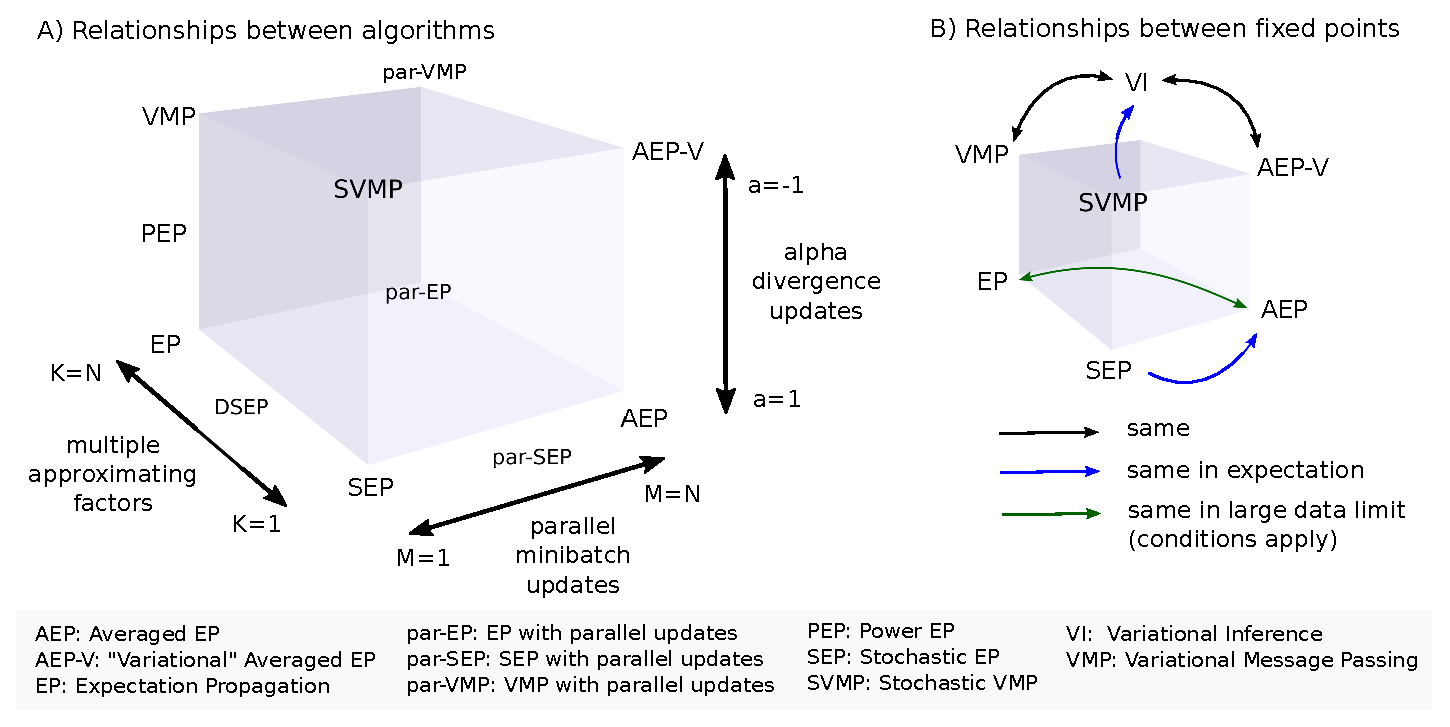
\includegraphics[height=6.5cm]{fig/relationship-algorithms.eps}%}
\caption{Relationships between algorithms. Note that care needs to be taken when interpreting the alpha-divergence as $a \rightarrow -1$ (see supplementary material).}
\label{fig:relationship-algorithms}
\end{figure}


%\section{Understanding stochastic expectation propagation}
In this section we provide theoretical understandings of stochastic EP, though the algorithm itself is motivated by practical computation issues. 

\subsection{Considering expectations of stochastic EP updates}
One important analysis of a stochastic algorithm is its dynamics in expectation, and the expectation of SEP's update step is the geometric average of new factors
$\bar{f}(\bm{\theta}) \propto [\prod_{i=1}^N f_i(\bm{\theta})]^{\frac{1}{N}}$.
This motivates the averaged EP (AEP) algorithm as the expectation version of stochastic EP, which performs almost the same computations, except that in the moment matching step it collects all the intermediate approximations $f_i(\bm{\theta}) \leftarrow \mathtt{proj}[\tilde{p}_i(\bm{\theta})] / q_{-1}(\bm{\theta})$ and use $\bar{f}(\bm{\theta})$ in the next inclusion step. 
%%%%
Unfortunately, finding out the loss function/free energy of AEP is not a trivial task. Instead we introduce a set of auxiliary distributions $\{q_i(\bm{\theta})\}$ and frame AEP as a double-loop algorithm. After the cavity computation step, the update $q(\bm{\theta})$ of AEP is constructed as follows:
%
\begin{itemize}
	\item \textbf{inner loop:} $q_i(\bm{\theta}) \leftarrow \arg\min_q KL(\tilde{p}_i(\bm{\theta}) ||q(\bm{\theta})) \buildrel\triangle\over = \mathtt{proj}[\tilde{p}_i(\bm{\theta})]$; 
	\item \textbf{outer loop:} $q(\bm{\theta}) \leftarrow \arg\min_q \sum_{i=1}^N KL(q(\bm{\theta}) ||q_i(\bm{\theta})) \buildrel\triangle\over = \mathtt{avg}[\{q_i(\bm{\theta})\}]$.
\end{itemize}
%
Note that the operator $\mathtt{avg}[\cdot]: \mathcal{Q}^N \rightarrow \mathcal{Q}$ can be defined on other distribution families similarly, and we abbreviate the formal definitions when re-introducing it later.
This framework allows us to analyse the convergence behaviour of AEP, where we have the following theorem.
%%%%%%%%%%%%%%%%%%%%%
\begin{theorem}
The fixed points of averaged EP, if exist, can be written as $q(\bm{\theta}) = \mathtt{avg}[\{q_i(\bm{\theta})\}]$, where
\begin{equation}
q_i(\bm{\theta}) = \mathtt{proj}[\tilde{p}_i(\bm{\theta})].
\label{eq:mm}
\end{equation}
These fixed points are also the fixed points of stochastic EP in expectation. 
\end{theorem}
\begin{proof}
In each update SEP gives the same answers as AEP in expectation if initialised at the same starting point. Also as an analogy to normal EP, the stationary points of AEP ask for moment matching between tilted and auxiliary distributions. 
\end{proof}
\textbf{Remark.} The convergence condition (\ref{eq:mm}) differs from the moment matching condition of full EP in that the matching requirements are proposed on the auxiliary distributions $\{q_i(\bm{\theta}) \}$ rather than the global approximation $q(\bm{\theta})$. The constraints are implicitly contained in the shared cavity distribution.

%
%
Averaged EP has also been proposed in \cite{barthelme:aep} but as a theoretical tool to study the convergence properties of normal EP. The authors showed that averaged EP can be interpreted as Newton methods in large data limit and proved the convergence chain EP $\rightarrow$ AEP $\rightarrow$ Newton in that case. However the results are very restrictive as it requires log-concave and very slow changing likelihood functions. 

\subsection{Connections to stochastic variational inference}
Applying stochastic optimisation to EP is also motivated by the great success of stochastic variational inference (SVI) \cite{hoffman:svi}. Both require memory allocation for global posterior only, compute updates based on the current sample, and perform updates with a suitable damping schedule. However SEP differs from SVI in the first view: the former processes local approximations, while the latter performs global optimisation. We attempt to connect SEP with SVI in a general framework, and we sketch two possible directions as local or global computation.

%
\textbf{Connecting SVI to a local optimisation algorithm.}
To understand SVI from a local optimisation perspective, consider VB as the expectation of SVI. We introduce a conceptual ``variational'' AEP by changing the moment matching step in the inner-loop to minimising the variational KL-divergence $KL(q_i(\bm{\theta}) || \tilde{p}_i(\bm{\theta}))$ wrt.~$q_i(\bm{\theta})$ \footnote{Also called information projection (I-projection) in \cite{amari:ig}).}. A similar version of EP is also presented in \cite{minka:divergence} as a special case of a generic message passing algorithm, where the author showed that EP with variational KL is equivalent to the variational message passing algorithm \cite{winn:vmp}. This result also applies to the ``variational'' AEP as the outer-loop computes a geometric average, with a formal proof in the supplementary material. 

%
\textbf{SEP in a global optimisation flavour.}
VB performs global optimisation on $KL(q(\bm{\theta})||p(\bm{\theta}|D))$, and its stochastic version, SVI, is driven by the gradients of $KL(q(\bm{\theta}) || p(\bm{\theta} | \{\bm{x}_i\}^N))$ on the $N$ replicates $\{\bm{x}_i\}^N$. Similarly, SEP computes a noisy estimation $q_i(\bm{\theta})$ by running the AEP inner-loop for the current sample only, though it is still a local optimisation at the first glance. However SEP can also be presented in a power EP (PEP) \cite{minka:powerep} fashion, if considering the likelihood term of $\bm{x}_i$ raised to power $N$ as the only factor. This allows us to state SEP as a stochastic global optimisation procedure, which minimises the $\alpha$-divergence \footnote{$D_{1}(p||q) \buildrel\triangle\over = KL(p || q) = \lim_{\alpha \rightarrow 1} D_{\alpha}(p||q)$, and $D_{ \mhyphen 1}(p||q) \buildrel\triangle\over = KL(q || p) = \lim_{\alpha \rightarrow \mhyphen 1} D_{\alpha}(p || q)$. } \cite{amari:ig1985}
\begin{equation}
D_{\alpha}(p(\bm{\theta} | \{\bm{x}_i\}^N) || q_i(\bm{\theta})) = \frac{4}{1 - \alpha^2} 
		\left( 1 - \int_{\bm{\theta}} p(\bm{\theta} | \{\bm{x}_i\}^N)^{(1 + \alpha) / 2} q_i(\bm{\theta})^{(1 - \alpha) / 2} d\bm{\theta} \right)
\end{equation} 
with $\alpha = \mhyphen 1 + 2/N$. Until now we managed to describe SVI and SEP in the same stochastic optimisation framework, which moves towards minimising $D(p(\bm{\theta} | \{\bm{x}_i\}^N), q(\bm{\theta}))$ for a given distance/divergence measure $D(\cdot, \cdot)$ on distributions. 

%
However applying this framework to the true posterior $p(\bm{\theta}|D)$ is often inconsistent with the expectation of stochastic optimisation. For the $\alpha$-divergence we selected, it recovers PEP on the whole dataset instead, and the factor to include in the tilted distribution changes to the intractable $\mathtt{avg}[\{p(\bm{x}_i | \bm{\theta}) \}]$. Readers might have noticed that the update of PEP on full dataset is given by $q(\bm{\theta}) \leftarrow \mathtt{proj}[\mathtt{avg}[\{ \tilde{p}_i(\bm{\theta}) \}]]$. In other words, we can restate the batch PEP algorithm by switching the order of M-projections and geometric averaging in AEP. Conversely we can interpret AEP as an approximation to the impractical batch PEP by interchanging computations. Figure \ref{fig:aep_vs_pep} illustrate a geometric view of this approximation, where the bias of this order swap is non-zero for most $D(\cdot, \cdot)$.

\subsection{Large-data limit revisited}
We provide a comparison between SEP and SVI in large-data limit using the global optimisation framework. We denote $\alpha \mhyphen \mathtt{proj}[p(\bm{\theta})]$ as the $\alpha$-projection \cite{amari:ig1985} \cite{amari:ig} of any distribution $p(\bm{\theta})$ to the $\mathcal{Q}$ family. Using this notation the previously defined $\mathtt{proj}[\cdot]$ operator is the $1$-projection, while SVI takes $\alpha = \mhyphen 1$. A similar analysis as \cite{amari:alpha_proj} indicates that in the large-data limit ($N \rightarrow \infty$), the $\alpha$-projection step obtains a minimiser of the variational $KL(q(\bm{\theta}) || p(\bm{\theta} | \{\bm{x}_i\}^N))$. However it does not necessary imply the equivalence between SEP and SVI since both algorithms in the inner-loop do not directly minimise their divergence objective. Instead they iteratively compute the current stochastic estimate $q_i(\bm{\theta})$ based on the previous solution, e.g.~line 4 in SEP Algorithm \ref{alg:sep}, and more importantly that iterative process is not continuous wrt.~$\alpha$ at $\alpha = -1$. Aslo the inner-loop divergences are very unlikely to reach their minimum as the outer loop violates the gradient descent computations. Further, even all of the auxiliary distributions converges to the local optima of the variational KL-divergences, there is no guarantee that the global approximation after averaging converges to a VB local optimum. A better restatement of SEP/AEP with infinite observations would be that SEP tends to behave like SVI when $N$ goes to infinity, although the connection of fixed point behaviour is still unclear. 

%
\begin{figure}
\centering
\def\svgwidth{0.35\linewidth}
\subfigure[\label{fig:aep_vs_pep}]{
\input{fig/aep_vs_pep.pdf_tex}}
%
\hspace{0.5in}
%
\def\svgwidth{0.4\linewidth}
\subfigure[\label{fig:dep_sep_dsep}]{
\input{fig/dep_sep_dsep.pdf_tex}}

\caption{(a) A geometric view of AEP/PEP comparison. (b) A cartoon illustration of DEP, SEP and DSEP. For each algorithm we show the approximate posterior on the top and the tilted distribution at the bottom.}

\end{figure}

%%%%%%%%%%%%%%%%%%%%%%%%%%%%%%%%%%%%%%%%%%%%%%%%%%%
%%%%%% SECTION 4: COMPUTATIONAL COMPLEXITY %%%%%
%
\section{Computational opportunities}

\subsection{Distributed Bayesian learning via data partitioning}
Recently distributed Bayesian computation methods have attracted significant amount of attentions \cite{broderick:stream}\cite{gelman:dep}\cite{xu:sms}, thanks to the advances of computation power and developments of parallel algorithms. The latter two papers proposed a distributed expectation propagation (DEP) framework, which first partitions the dataset into $K$ disjoint pieces $\{ D_k = \{\bm{x}_i\}_{i=1}^{N_k} \}$ with $N = \sum_{i=1}^K N_k$, then assigns factors to each sub-datasets. The projection step is computed by sampling methods, making DEP stochastic in the sense of moment approximation. SEP/AEP can be incorporated into this framework as well, where we present the two different opportunities as follows and provide a cartoon view in Figure \ref{fig:dep_sep_dsep}.

\textbf{SEP/AEP outside minibatches.} We tie all the factors on minibatches and run SEP/AEP accordingly. The fraction we exclude/include changes to $1/K$, and the moment computation is by advance sampling methods. Notice that the procedure is doubly stochastic when running SEP on this. Also AEP can be very accurate but with the price of much slower computation as it waits for sampling procedure on each minibatch to finish.

\textbf{SEP/AEP inside minibatches.} Distributed EP might be preferred in practice if storing local factors is affordable. However compared to sampling approaches that is generally time consuming, running SEP/AEP inside each minibatch can achieve significant speed-up if there exists a closed-form solution. Now the scaling fraction of the algorithm turns out to be $1/N_k$ when updating the $k^{th}$ site, and the cavity computation changes to $q(\bm{\theta})_{-k} \propto q(\bm{\theta}) / f_k(\bm{\theta})^{1 / N_k}$. We refer this type of SEP/AEP as DSEP/DAEP in the rest of the paper.

%%%%%%
\subsection{Complexity comparisons}
We examine the computational gains of SEP/AEP in detail and compare them with other EP-like algorithms in literature. Candidate methods include normal EP, stochastic EP, average EP, distributed EP, and the potentially flawed assumed density filtering for multiple passes. Note that AEP and DEP are trivial to go parallel, where for simplicity we neglect the transmission expense. We also assume Gaussian approximations for the posterior and an equal partitioning of the dataset.

%%%
We start from the optional data partitioning step with instant cost. Next we initialise the global (and local) factors, requiring $\mathcal{O}(Kd^2)$ memory spaces for normal EP and DEP, and $\mathcal{O}(d^2)$ for the others. All EP algorithms except ADF proceed to compute the cavity distribution in $\mathcal{O}(d^3)$ time for each local factors. The tilted distributions are then conceptually formed for analytical/stochastic moment computation with cost defined as $\mathcal{O}(h(n, d))$ each, where $n$ is the number of datapoints involved in the local posterior. Such complexity includes $\mathcal{O}(d^3)$ for matrix inversion and/or $ >> \mathcal{O}(d^2)$ for sampling methods. The complexity of inclusion is $\mathcal{O}(d^2)$ for a single update, but the total number of updates in one full pass varies for different algorithms. AEP and DEP incorporate the local factors only after the full pass, while the others modify the global approximation after processing each site. However when parallel, it might be sensible to include updates according to a schedule if parameter transmission cost is large.

%%%
We list the space and time complexity factors of several algorithms in Table \ref{table:complexity}. The figures apply to fully observed models, while none of them have advantage on the others on local hidden variable posterior approximations. Like the comparison between batch and stochastic learning methods, AEP produces more robust updates, and can be significantly faster than SEP when parallel. However AEP requires more passes of datasets than SEP, which might be a problem when with limited computation time. On the other hand, SEP might be too noisy, so SEP with minibatch averaging is preferred in general.

\begin{table}[t]
\caption{Complexity figures for the EP algorithms discussed. The time complexities are counted on a full pass of dataset, and the global approximations are updated after each moment computation. }
\label{table:complexity}
\begin{center}
\begin{tabular}{lll}
\multicolumn{1}{c}{\bf Type}  &\multicolumn{1}{c}{\bf Time complexity} &\multicolumn{1}{c}{\bf Space complexity}
\\ \hline 
Normal EP         		&$\mathcal{O}(K(d^3 + h(N/K, d) + d^2))$ 		&$\mathcal{O}(Kd^2)$ \\
Distributed EP        	&$\mathcal{O}(d^3 + h(N/K, d) + d^2)$			&$\mathcal{O}(Kd^2)$ \\
Averaged EP (sequel)     &$\mathcal{O}(d^3 + K h(N/K, d) + d^2)$ 		&$\mathcal{O}(d^2)$ \\
Averaged EP (parallel)   &$\mathcal{O}(d^3 + h(N/K, d) + d^2)$ 		&$\mathcal{O}(Kd^2)$ \\
Stochastic EP 			&$\mathcal{O}(K(d^3 + h(N/K, d) + d^2))$ 		&$\mathcal{O}(d^2)$ \\
ADF (multi.~pass) 		&$\mathcal{O}(K(h(N/K, d) + d^2))$ 		&$\mathcal{O}(d^2)$ \\
\hline
Sampling 				&$\mathcal{O}(h(N, d))$			&$\mathcal{O}(d^2)$
\end{tabular}
\end{center}
\end{table}

%%%%%%%%%%%%%%%%%%%%%%%%%%%%%%%%%%%%%%%%%%%%%%%%%%
%%%%% SECTION 5: EXPERIMENTS %%%%%%%%%%%%%%%%%
\section{Experiments}
%%%%%%%%%%%% SYNTHETIC %%%%%%%%%%%%
%We evaluate SEP on both synthetic and real-world data, and for brevity we omit the mathematical details. In synthetic tests we compare the approximations against the true posterior constructed by No-U-Turn sampler (NUTS) \cite{hoffman:nuts} implemented in \texttt{stan}\footnote{\url{http://mc-stan.org/pystan.html}}. We repeat all tests for 5 times.
%%
%For real datasets we test classification tasks with probit regression. We further conduct regression tasks using neural networks trained with probabilistic back-propagation \cite{miguel:pbp}, which is based on ADF in the first place. We modify the available code\footnote{\url{https://github.com/HIPS/Probabilistic-Backpropagation}} to support full EP and SEP training and compare their performances to the reported ADF results.

The purpose of the experiments was to evaluate SEP on a number of datasets (synthetic and real-world, small and large) and on a number of models (probit regression, Mixture of Gaussians and Bayesian neural networks).

%%%% SECOND EXAMPLE %%%%
\subsection{Bayesian Probit Regression}
%
The first experiments considered a simple Bayesian classification problem and investigated the stability and quality of SEP in relation to EP and ADF as well as the effect of using mini-batches and varying the granularity of the approximation. The model comprised a probit likelihood function $P(\bm{y}_n = 1|\theta) = \Phi(\bm{\theta}^T \bm{x}_n)$ and a Gaussian prior over the hyper-plane parameter  $p(\bm{\theta}) = \mathcal{N}(\bm{\theta}; \bm{0}, 1.5^2 I)$.  

The first experiments used synthetic data comprised $N=5,000$ datapoints $\{ (\bm{x}_n, \bm{y}_n) \}$. The inputs $\bm{x}_n$ were $D=4$ dimensional and were either sampled from a single Gaussian distribution (Fig.~\ref{fig:sep_probit}a) or from a Mixture of Gaussians (MoGs) with $J=5$ components (Fig.~\ref{fig:sep_probit}b) to investigate the sensitivity of the methods to the homogeneity of the dataset. The labels were produced by sampling from the generative model. Performance was measured by computing an approximation of $\mathrm{KL}(p(\bm{\theta}|\mathcal{D}) || q(\bm{\theta}))$ where $p(\bm{\theta}|\mathcal{D})$ was replaced by a Gaussian that had the same mean and covariance as samples drawn from the posterior using the No-U-Turn sampler (NUTS) \cite{hoffman:nuts}.

 %The binary labels $\bm{y}_n$ are sampled from a Probit unit with a hyper-plane sampled from a Gaussian $\bm{\theta}_{true} \sim \mathcal{N}(\bm{\theta}; \bm{0}, I)$. For learning we use a Gaussian prior and measure the

Results in Figure \ref{fig:sep_probit} indicate that EP is the best performing method and that ADF collapses towards a delta function at the posterior mean as expected. SEP converges to a solution which appears to be of similar quality to that obtained by EP for the dataset containing Gaussian inputs, but slightly worse when the MoGs was used. Variants of SEP that used larger mini-batches fluctuated less, but typically took longer times to converge.\todo[fancyline]{From the fig (a) -- looks like larger M is faster?!} The utility of finer grained approximations depended on the homogeneity of the data. For the dataset containing Gaussian inputs increasing the number of approximation factors from $K=1$ (SEP) to $K=50$ (DAEP) provided no advantage. However, for the second dataset containing MoG inputs, finer grained approximations were found to be advantageous if the datapoints from each mixture component are assigned to the same approximating factor. Generally it was found that there is no advantage to retaining more approximating factors than there were clusters in the dataset.  

%We change the simulation model of $\bm{x}$ to a mixture of $J=5$ Gaussians, and partition the datasets into $K$ minibatches with datapoints from the same cluster. Figure \ref{fig:daep_probit} shows that SEP converges to slightly worse approximations as it only maintains the global posterior. In contrast DAEP performs nearly identical to full EP in convergence. The number of factors $K$ has little effect on the performance once $K \geq J$, indicating that the contributions of datapoints in the same cluster are very similar. 

To verify whether these conclusions about the granularity of the approximation hold in real datasets, we sampled $N=1,000$ datapoints for each of the digits in MNIST and performed odd-vs-even classification. Each digit class was assigned its own global approximating factor, $K=10$. We compare the log-likelihood of a test set using ADF, SEP ($K=1$), full EP and DSEP ($K=10$) in Figure \ref{fig:mnist}. EP and DSEP significantly outperform ADF. DSEP is slightly worse than full EP initially, however it reduces the memory to 0.001\% of full EP without losing substantial accuracy. SEP's performance was still increasing at the end of learning and was slightly better than ADF.

Finally, we tested SEP's performance on six small binary classification datasets from the UCI machine learning repository.\footnote{\url{https://archive.ics.uci.edu/ml/index.html}} We did not consider the effect of mini-batches or the granularity of the approximation, using $K=M=1$. The classification results are summarised in Table \ref{tab:probit_results}. ADF performed reasonably well on the root mean square error (RMSE) metric, presumably because it tends to learn a good approximation to the posterior mode. However, the posterior variance is poorly approximated and therefore ADF returns poor test log-likelihood scores. EP achieves significantly higher test log-likelihood than ADF indicating that a superior approximation to the posterior variance is attained. Crucially, SEP performs very similarly to EP, implying that SEP is an accurate alternative to EP even though it is refining a cheaper global posterior approximation.\todo[fancyline]{mention N here and the memory saving?}

\begin{figure}
\centering
\def\svgwidth{0.31\linewidth}
\subfigure[\label{fig:sep_probit}]{
\input{fig/sep_probit.pdf_tex}}
%
%\hspace{0.01in}
%
\def\svgwidth{0.31\linewidth}
\subfigure[\label{fig:daep_probit}]{
\input{fig/daep.pdf_tex}}
%
%\hspace{0.01in}
%
\def\svgwidth{0.31\linewidth}
\subfigure[\label{fig:mnist}]{
\input{fig/mnist_error.pdf_tex}}
\caption{Bayesian logistic regression experiments. Panels (a) and (b) show synthetic data experiments. Panel (c) shows the results on MNIST (see text for full details)}
\end{figure}

\begin{table} 
\small
\centering \label{tab:probit_results} \begin{tabular}{l@{\ica}r@{$\pm$}l@{\ica}r@{$\pm$}l@{\ica}r@{$\pm$}l@{\ica}r@{$\pm$}l@{\ica}r@{$\pm$}
	l@{\ica}r@{$\pm$}l@{\ica}r@{$\pm$}}\hline 
{} & \multicolumn{6}{c}{RMSE} & \multicolumn{6}{c}{test log-likelihood} \\
\bf{Dataset}&\multicolumn{2}{c}{\bf{ ADF }}&\multicolumn{2}{c}{\bf{ SEP }}&\multicolumn{2}{c}{\bf{ EP }} &\multicolumn{2}{c}{\bf{ ADF }}&\multicolumn{2}{c}{\bf{ SEP }}&\multicolumn{2}{c}{\bf{ EP }} \\ \hline 
%
Australian&0.328&0.0127&\bf{0.325}&\bf{0.0135}&0.330&0.0133
	&-0.634&0.010&-0.631&0.009&\bf{-0.631}&\bf{0.009}\\
%
Breast&0.037&0.0045&\bf{0.034}&\bf{0.0034}&0.034&0.0039
	&-0.100&0.015&-0.094&0.011&\bf{-0.093}&\bf{0.011}\\
%
Crabs&0.062&0.0125&\bf{0.040}&\bf{0.0106}&0.048&0.0117
	&-0.290&0.010&\bf{-0.177}&\bf{0.012}&-0.217&0.011\\
%
Ionos&\bf{0.126}&\bf{0.0166}&0.130&0.0147&0.131&0.0149
	&-0.373&0.047&-0.336&0.029&\bf{-0.324}&\bf{0.028}\\
%
Pima&0.242&0.0093&0.244&0.0098&\bf{0.241}&\bf{0.0093}
	&-0.516&0.013&-0.514&0.012&\bf{-0.513}&\bf{0.012}\\
%
Sonar&\bf{0.198}&\bf{0.0208}&0.198&0.0217&0.198&0.0243
	&-0.461&0.053&-0.418&0.021&\bf{-0.415}&\bf{0.021}\\
 \hline \end{tabular} 
 \caption{ Average test results all methods on Probit regression. All methods capture a good posterior mean, however EP outperforms ADF in terms of test log-likelihood on almost all the datasets, with SEP performing similarly to EP.}
 \end{table} 
 
 %
%%%% FIRST EXAMPLE %%%%
\subsection{Mixture of Gaussians for Clustering}
%
The small scale experiments on probit regression indicate that SEP performs well for fully-observed probabilistic models. Although it is not the main focus of the paper, we sought to test the flexibility of the method by applying it to a latent variable model, specifically a Mixture of Gaussians. A synthetic MoGs dataset containing $N=200$ datapoints was constructed comprising $J=4$ Gaussians. The means were sampled from a Gaussian distribution, $p(\bm{\mu}_j)= \mathcal{N}(\bm{\mu}; \bm{m}, \mathrm{I})$, the cluster identity variables were sampled from a uniform categorical distribution $p(\bm{h}_n = j) = 1/4$, and each mixture component was isotropic $p(\bm{x}_n | \bm{h}_n) = \mathcal{N}(\bm{x}_n; \bm{\mu}_{\bm{h}_n}, 0.5^2 I)$. EP, ADF and SEP were performed to approximate the joint posterior over the cluster means $\{ \bm{\mu}_j\}$ and cluster identity variables $\{ \bm{h}_n \}$ (the other parameters were assumed known). 

%EP, SEP and ADF are applied to approximate the posterior of $\bm{\theta} = \{ \bm{\mu}_j \}$ with Gaussians and $\{\bm{h}_n\}$ with categorical distributions, though the storage for the latter terms is not required. 

Figure \ref{fig:gmm_visualised} visualises the approximate posteriors after 200 iterations. All methods return good estimates for the means, but ADF collapses towards a point estimate as expected. SEP, in contrast, captures the uncertainty and returns nearly identical approximations to EP. The accuracy of the methods is quantified in Fig.~\ref{fig:gmm_error} by comparing the approximate posteriors to those obtained from the No-U-Turn sampler. These measures confirm that SEP approximates EP well.

\begin{figure}
\centering
\def\svgwidth{0.50\linewidth}
\subfigure[\label{fig:gmm_visualised}]{
\input{fig/gmm1.pdf_tex}}
%
\hspace{0.1in}
%
\def\svgwidth{0.40\linewidth}
\subfigure[\label{fig:gmm_error}]{
\input{fig/gmm_error.pdf_tex}}
\caption{Posterior approximation for the mean of the Gaussian components. (a) shows posterior approximations over the cluster means (98\% confidence level). The coloured dots indicate the true label (top-left) or the inferred cluster assignments (the rest). In (b) we show the error of the approximations as measured by the averaged Frobenius norm of the difference between the the closest means posterior samples and EP approximations, mean (top) and covariance (bottom).}
\end{figure}


%%%%%%%%%%%% PBP %%%%%%%%%%%
\subsection{Probabilistic back-propagation}

Probabilistic-backpropagation (PBP) \cite{hernandez2015probabilistic} is a
recent state-of-the-art method for scalable approximate inference in neural
network models. PBP works by doing several iterations of ADF over the training
data.  The moment-matching operations required by ADF are computed by
first propagating the uncertainty on the synaptic weights forward through the network
and then computing the gradient of the marginal likelihood by backpropagation.
PBP is based on ADF to reduce the large memory cost that would be required by EP
when the amount of available data is very large.

We performed several experiments to asses the accuracy of different implementations of PBP
based on ADF, SEP and EP. We considered neural networks with 100 hidden units and followed the same experimental protocol 
as the one described by \cite{hernandez2015probabilistic}.
Table 2 shows the average test RMSE and test log-likelihood for each method.
Interestingly, SEP and ADF often outperform EP in this case.
Finally, Table 3 shows the reduction in memory consumption when SEP is compared with EP.
This reduction scales as a function of the dataset size and for the biggest
one, Year, it is of several tens of gigabytes.
 
\begin{table} 
\small
\centering \caption{ Average test results all methods. } \label{tab:results} \begin{tabular}{l@{\ica}r@{$\pm$}l@{\ica}r@{$\pm$}l@{\ica}r@{$\pm$}l@{\ica}r@{$\pm$}l@{\ica}r@{$\pm$}l@{\ica}r@{$\pm$}l@{\ica}r@{$\pm$}}\hline 
{} & \multicolumn{6}{c}{RMSE} & \multicolumn{6}{c}{test log-likelihood} \\
\bf{Dataset}&\multicolumn{2}{c}{\bf{ ADF }}&\multicolumn{2}{c}{\bf{ SEP }}&\multicolumn{2}{c}{\bf{ EP }} &\multicolumn{2}{c}{\bf{ ADF }}&\multicolumn{2}{c}{\bf{ SEP }}&\multicolumn{2}{c}{\bf{ EP }} \\ \hline 
%
Kin8nm&0.098&0.0007&\bf{0.088}&\bf{0.0009}&0.089&0.0006
	&0.896&0.006&\bf{1.013}&\bf{0.011}&1.005&0.007\\ 
%
Naval&0.006&0.0000&\bf{0.002}&\bf{0.0000}&0.004&0.0000
	&3.731&0.006&\bf{4.590}&\bf{0.014}&4.207&0.011\\  
%
Power&\bf{4.124}&\bf{0.0345}&4.165&0.0336&4.191&0.0349
	&\bf{-2.837}&\bf{0.009}&-2.846&0.008&-2.852&0.008\\
% 
Protein&4.727&0.0112&\bf{4.670}&\bf{0.0109}&4.748&0.0137
	&-2.973&0.003&\bf{-2.961}&\bf{0.003}&-2.979&0.003\\ 
%
Wine&\bf{0.635}&\bf{0.0079}&0.650&0.0082&0.637&0.0076
	&-0.968&0.014&-0.976&0.013&\bf{-0.958}&\bf{0.011}\\  
%
Year&\bf{8.879}&\bf{   NA}&8.922&   NA&8.914&   NA
&\bf{-3.603}&\bf{  NA}&-3.924&  NA&-3.929&  NA\\
 \hline \end{tabular} \end{table} 


\begin{table} 
%\begin{minipage}[!t]{0.6\linewidth}
\small
\centering 
\begin{tabular}{lrrr}\hline \bf{Dataset}& $N$ & $d$ & MB reduced\\ \hline 
Kin8nm & 8,192 & 8 & 58.46MB \\ 
Naval & 11,934 & 16 & 147.84MB\\ 
Power Plant & 9,568 & 4 & 37.98MB\\ 
Protein & 45,730 & 9 & \bf{694.02MB}\\ 
Wine & 1,599 & 11 & 14.30MB\\ 
Year & 515,340 & 90 & \bf{65107.34MB}\\ \hline 
\end{tabular} 
\caption{ Memory reduction of SEP from full EP. } \label{tab:memory} 
%\end{minipage}
\end{table} 
%
%\begin{minipage}[!t]{0.35\linewidth}
%\begin{figure}

%\centering
%\def\svgwidth{0.9\linewidth}
%\subfigure[\label{fig:sonar}]{
%\input{fig/sonar.pdf_tex}}
%\caption{Averaged test likelihood for long-time training.}

%\end{figure}
%\end{minipage}


%%%%%%%%%%%%%%%%%%%%%%%%%%%%%%%%%%%%%%%%%%%%%%%%%%
%%%%%%%%%%%% SECTION 6: CONCLUTIONS %%%%%%%%%%%%%%
\section{Conclusions and future work}
This paper has presented the stochastic expectation propagation method for reducing EP's large memory consumption which is often prohibitive for large datasets. We have connected the new algorithm to a number of existing methods including assumed density filtering, variational message passing, variational inference, stochastic variational inference and averaged EP.
%
Experiments on Bayesian logistic regression (both synthetic and real world) and mixture of Gaussians clustering indicated that the new method had an accuracy that was competitive with EP.  Experiments on the probabilistic back-propagation on large real world regression datasets again showed that SEP comparably to EP with a vastly reduced memory footprint. 
%
Future experimental work will focus on developing data-partitioning methods to leverage finer-grained approximations (DESP) that showed promising experimental performance and also mini-batch updates. There is also a need for further theoretical understanding of both the new algorithms and EP itself as well as systematic empirical comparisons of EP-like algorithms and variational methods to guide the practitioners when they select an approximation scheme.


\subsubsection*{References}
\renewcommand{\section}[2]{}
\bibliographystyle{unsrt}
\bibliography{nips_sep}


\end{document}
